%%%%%%%%%%%%%%%%%%%%%%%%%%%%%%%%%%%%%%%%%
% Make sure to set your name, legi number and url to the right git branch.
\newcommand{\hmwkAuthorName}{Michael Sch\"{u}rch} % Your name
\newcommand{\hmwkAuthorLegi}{13-916-614} % Your Legi
\newcommand{\hmwkGitBranch}{13-916-614/1\_locally\_linear\_embedding} % your git branch
%
%%%%%%%%%%%%%%%%%%%%%%%%%%%%%%%%%%%%%%%%%

%----------------------------------------------------------------------------------------
%	PACKAGES AND OTHER DOCUMENT CONFIGURATIONS
%	Skip this
%----------------------------------------------------------------------------------------

\documentclass{article}

\usepackage{fancyhdr} % Required for custom headers
\usepackage{lastpage} % Required to determine the last page for the footer
\usepackage{extramarks} % Required for headers and footers
\usepackage{graphicx} % Required to insert images
\usepackage{lipsum} % Used for inserting dummy 'Lorem ipsum' text into the template
\usepackage{subcaption}

% Margins
\topmargin=-0.45in
\evensidemargin=0in
\oddsidemargin=0in
\textwidth=6.5in
\textheight=9.0in
\headsep=0.25in 

\linespread{1.1} % Line spacing

% Set up the header and footer
\pagestyle{fancy}
\lhead{\hmwkAuthorName} % Top left header
\chead{\hmwkClass\ \hmwkTitle} % Top center header
\rhead{\firstxmark} % Top right header
\lfoot{\lastxmark} % Bottom left footer
\cfoot{} % Bottom center footer
\rfoot{Page\ \thepage\ of\ \pageref{LastPage}} % Bottom right footer
\renewcommand\headrulewidth{0.4pt} % Size of the header rule
\renewcommand\footrulewidth{0.4pt} % Size of the footer rule

\setlength\parindent{0pt} % Removes all indentation from paragraphs

%----------------------------------------------------------------------------------------
%	DOCUMENT STRUCTURE COMMANDS
%	Skip this
%----------------------------------------------------------------------------------------

% Header and footer for when a page split occurs within a problem environment
\newcommand{\enterProblemHeader}[1]{
\nobreak\extramarks{#1}{#1 continued on next page\ldots}\nobreak
\nobreak\extramarks{#1 (continued)}{#1 continued on next page\ldots}\nobreak
}

% Header and footer for when a page split occurs between problem environments
\newcommand{\exitProblemHeader}[1]{
\nobreak\extramarks{#1 (continued)}{#1 continued on next page\ldots}\nobreak
\nobreak\extramarks{#1}{}\nobreak
}

\setcounter{secnumdepth}{0} % Removes default section numbers
\newcounter{homeworkProblemCounter} % Creates a counter to keep track of the number of problems

\newcommand{\homeworkProblemName}{}
\newenvironment{homeworkProblem}[1][Problem \arabic{homeworkProblemCounter}]{ % Makes a new environment called homeworkProblem which takes 1 argument (custom name) but the default is "Problem #"
\stepcounter{homeworkProblemCounter} % Increase counter for number of problems
\renewcommand{\homeworkProblemName}{#1} % Assign \homeworkProblemName the name of the problem
\section{\homeworkProblemName} % Make a section in the document with the custom problem count
\enterProblemHeader{\homeworkProblemName} % Header and footer within the environment
}{
\exitProblemHeader{\homeworkProblemName} % Header and footer after the environment
}

\newcommand{\problemAnswer}[1]{ % Defines the problem answer command with the content as the only argument
\noindent\framebox[\columnwidth][c]{\begin{minipage}{0.98\columnwidth}#1\end{minipage}} % Makes the box around the problem answer and puts the content inside
}

\newcommand{\homeworkSectionName}{}
\newenvironment{homeworkSection}[1]{ % New environment for sections within homework problems, takes 1 argument - the name of the section
\renewcommand{\homeworkSectionName}{#1} % Assign \homeworkSectionName to the name of the section from the environment argument
\subsection{\homeworkSectionName} % Make a subsection with the custom name of the subsection
\enterProblemHeader{\homeworkProblemName\ [\homeworkSectionName]} % Header and footer within the environment
}{
\enterProblemHeader{\homeworkProblemName} % Header and footer after the environment
}
   
%----------------------------------------------------------------------------------------
%	NAME AND CLASS SECTION
%	Skip this
%----------------------------------------------------------------------------------------

\newcommand{\hmwkTitle}{Locally Linear Embedding} % Assignment title
\newcommand{\hmwkDueDate}{Monday,\ March\ 6th,\ 2017} % Due date
\newcommand{\hmwkClass}{SLT coding exercise\ \#1} % Course/class
\newcommand{\hmwkClassTime}{Mo 16:15} % Class/lecture time
\newcommand{\hmwkClassInstructor}{} % Teacher/lecturer

%----------------------------------------------------------------------------------------
%	TITLE PAGE
%	Skip this
%----------------------------------------------------------------------------------------

\title{
\vspace{2in}
\textmd{\small{\hmwkClass}}\\
\textmd{\textbf{\hmwkTitle}}\\
\small{https://gitlab.vis.ethz.ch/vwegmayr/slt-coding-exercises}\\
\normalsize\vspace{0.1in}\small{Due\ on\ \hmwkDueDate}
%\vspace{0.1in}\large{\textit{\hmwkClassInstructor\ \hmwkClassTime}}
\vspace{3in}
}

\author{
\hmwkAuthorName\\
\hmwkAuthorLegi
}

\date{ } % Insert date here if you want it to appear below your name

\begin{document}

\maketitle

%----------------------------------------------------------------------------------------
%	TABLE OF CONTENTS
%	Skip this
%----------------------------------------------------------------------------------------

%\setcounter{tocdepth}{1} % Uncomment this line if you don't want subsections listed in the ToC

\newpage
\tableofcontents
\newpage

%----------------------------------------------------------------------------------------
%	SECTIONS
%	Now you are in the right hood
%----------------------------------------------------------------------------------------

\begin{homeworkProblem}[The Model]
%The model section is intended to allow you to recapitulate the essential ingredients used in \hmwkTitle. Write down the \textit{necessary} equations to specify \hmwkTitle\ and and shortly explain the variables that are involved. This section should only introduce the equations, their solution should be outlined in the implementation section.\newline
%Hard limit: One page
%\vspace{10pt}
\problemAnswer{ % Answer
The LLE algorithm is a method for dimensionality reduction in an unsupervised manner. Thus for some data matrix $\mathcal{X} \in \mathbf{R}^{nxD}$ with n data points of size D we seek a new matrix $\mathcal{Y} \in \mathbf{R}^{nxd}$ with $d < D$ thus reducing the dimension of each data point. \\

The objective of LLE is to minimize the following reconstruction error:

$$ \mathcal{E}(W) = \sum_{i}\big|X_i - \sum_{j}W_{ij}X_j\big|^2$$

where we have the constraint that $\sum_{j}W_{ij}=1$ and $W_{ij}=0$ if $X_j$ isn't one of the K closest neighbors of $X_i$. \\

In a final step we use found $W$ and map every high dimensional observation $X_i$ to a low dimensional vector $Y_i$. This is done by minimizing the embedding cost function:

$$ \Phi(Y) = \sum_{i}\big|Y_i - \sum_{j}W_{ij}Y_j\big|^2 = \sum_{ij}M_{ij}(Y_i \cdot Y_j)$$

with the constraint that $\sum_{i}Y_i = 0$ and $\frac{1}{N}\sum_{i} Y_i Y_i^T = I$
\\\\\\\\\\\\\\\\\\\
This information was gathered from https://www.cs.nyu.edu/~roweis/lle/papers/lleintro.pdf.

}





%\problemAnswer{ % Answer
%Your Answer
%}
\end{homeworkProblem}
\clearpage

%----------------------------------------------------------------------------------------
\begin{homeworkProblem}[The Questions - solved]
%This is the core section of your report, which contains the tasks for this exercise and your respective solutions. Make sure you present your results in an illustrative way by making use of graphics, plots, tables, etc. so that a reader can understand the results with a single glance. Check that your graphics have enough resolution or are vector graphics. Consider the use of GIFs when appropriate.\newline
%Hard limit: Two pages

\problemAnswer{
	

\begin{homeworkSection}{(a) Get the data}
%For this exercise we will work with the MNIST data set. In order to learn more about it and download it, go to http://yann.lecun.com/exdb/mnist/.
%I got the data from http://yann.lecun.com/exdb/mnist/ and uncompressed it into the folder /data. I did not include the data into the commit because I think that would be bad practice (if everybody does it alot of redundancy)
I got the data from http://yann.lecun.com/exdb/mnist/ and uncompressed it into the folder ./data. 
\end{homeworkSection}

}
\problemAnswer{
\begin{homeworkSection}{(b) Locally linear embedding}
%Implement the LLE algorithm and apply it to the MNIST data set. Provide descriptive visualizations for 2D \& 3D embedding spaces. Is it possible to see clusters?
For the 2D embedding space we can observe that the numbers 1 and 0 form a cluster and all other numbers seem to be scrambled into a third cluster in the middle. The 3D embedding space additionally manages to distinguish between numbers 6,2 and 7,4.

\end{homeworkSection}
}
\begin{figure}[h]
	\centering
	\begin{subfigure}[b]{0.44\textwidth}
		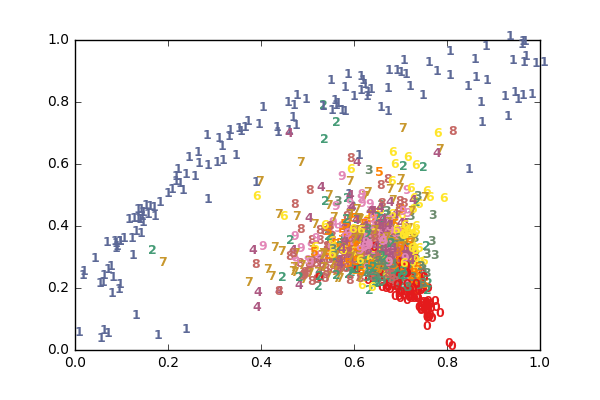
\includegraphics[width=\textwidth]{src/fig30_2.png}
		\caption{2D LLE plot}
		\label{fig:src/1fig30_2.png}
	\end{subfigure}
	~ %add desired spacing between images, e. g. ~, \quad, \qquad, \hfill etc. 
	%(or a blank line to force the subfigure onto a new line)
	\begin{subfigure}[b]{0.49\textwidth}
		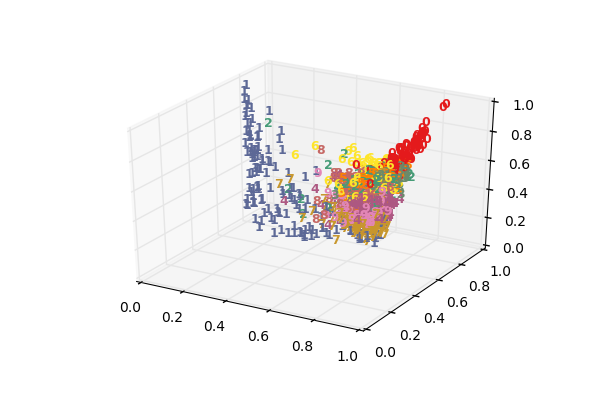
\includegraphics[width=\textwidth]{src/fig30_3.png}
		\caption{3D LLE plot}
		\label{fig:src/1fig30_3.png}
	\end{subfigure}
	~ %add desired spacing between images, e. g. ~, \quad, \qquad, \hfill etc. 
	%(or a blank line to force the subfigure onto a new line)
	\caption{}\label{fig:fig1}
\end{figure}


\problemAnswer{
\begin{homeworkSection}{(c) Cluster structure}
%Investigate the cluster structure of the data. Can you observe block structures in the $M$ matrix (use matrix plots)? Also plot the singular values of $M$. Do you notice something?
%Can you think of ways to determine the optimal embedding dimension?

The matrix $M$, see Fig. \ref{fig:src/1figM.png}, is very sparse. It also has most of its non-zero entries on its diagonal and is symmetric. But I cannot see any form of a block structure. The singular values of $M$ can be seen in Fig. \ref{fig:src/1figEV.png}. As of determining the optimal embedding dimension we can basically read off the reconstruction error by summing up the last d eigenvalues. Therefore we can estimate the error easily and choose a certain threshold.

\end{homeworkSection}
}

\begin{figure}[h]
	\centering
	\begin{subfigure}[b]{0.32\textwidth}
		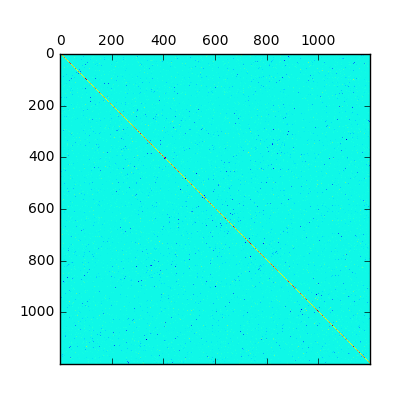
\includegraphics[width=\textwidth]{src/figM.png}
		\caption{The $M$ matrix}
		\label{fig:src/1figM.png}
	\end{subfigure}
	~ %add desired spacing between images, e. g. ~, \quad, \qquad, \hfill etc. 
	%(or a blank line to force the subfigure onto a new line)
	\begin{subfigure}[b]{0.45\textwidth}
		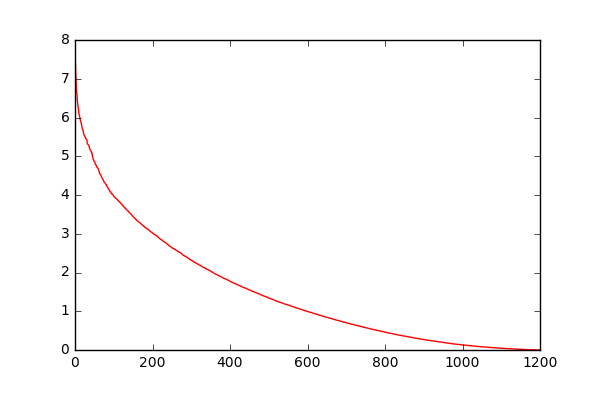
\includegraphics[width=\textwidth]{src/figEV.png}
		\caption{singular values of $M$}
		\label{fig:src/1figEV.png}
	\end{subfigure}
	~ %add desired spacing between images, e. g. ~, \quad, \qquad, \hfill etc. 
	%(or a blank line to force the subfigure onto a new line)
	\caption{}\label{fig:fig2}
\end{figure}
\newpage

\problemAnswer{
\begin{homeworkSection}{(d) Nearest Neighbors}
%Investigate the influence of the choice of how many nearest neighbors you take into account. Additionally, try different metrics to find the nearest neighbors (we are dealing with images!).
As can be seen in the following illustrations Fig \ref{fig:fig3}, \ref{fig:fig4} the choice of K and the metric can have a big effect on the quality of the solution.

\end{homeworkSection}
}

\begin{figure}[h]
	\centering
	\begin{subfigure}[b]{0.28\textwidth}
		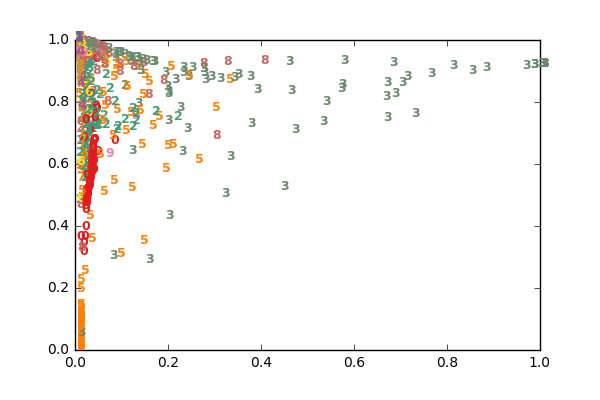
\includegraphics[width=\textwidth]{src/fig5_minkowski.png}
		\caption{LLE with K = 5}
		\label{fig:src/1figMinkovski5.png}
	\end{subfigure}
	~ %add desired spacing between images, e. g. ~, \quad, \qquad, \hfill etc. 
	%(or a blank line to force the subfigure onto a new line)
	\begin{subfigure}[b]{0.28\textwidth}
		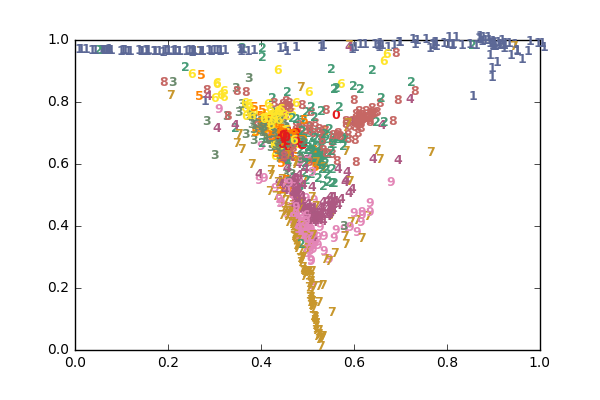
\includegraphics[width=\textwidth]{src/fig10_minkowski.png}
		\caption{LLE with K = 10}
		\label{fig:src/1figMinkovski10.png}
	\end{subfigure}
	%(or a blank line to force the subfigure onto a new line)
	\begin{subfigure}[b]{0.28\textwidth}
		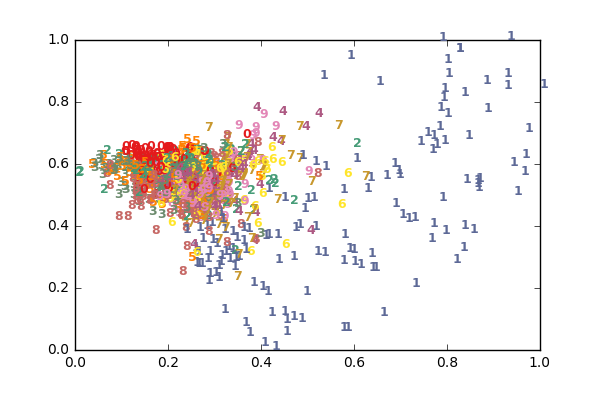
\includegraphics[width=\textwidth]{src/fig50_minkowski.png}
		\caption{LLE with K = 50}
		\label{fig:src/1figMinkovski50.png}
	\end{subfigure}
	~ %add desired spacing between images, e. g. ~, \quad, \qquad, \hfill etc. 
	%(or a blank line to force the subfigure onto a new line)
	\caption{Minkovski metric}\label{fig:fig3}
\end{figure}

\begin{figure}[h]
	\centering
	\begin{subfigure}[b]{0.28\textwidth}
		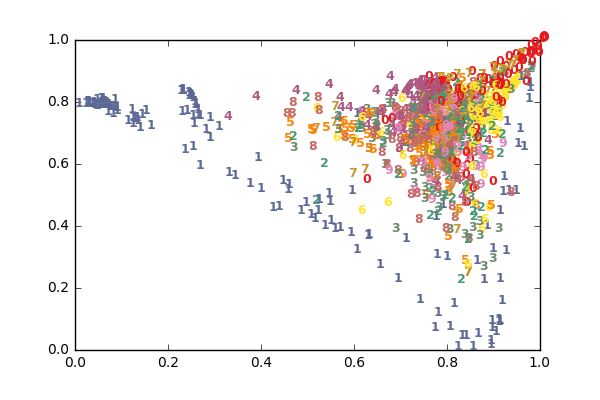
\includegraphics[width=\textwidth]{src/fig5_chebyshev.png}
		\caption{LLE with K = 5}
		\label{fig:src/1figCheby5.png}
	\end{subfigure}
	~ %add desired spacing between images, e. g. ~, \quad, \qquad, \hfill etc. 
	%(or a blank line to force the subfigure onto a new line)
	\begin{subfigure}[b]{0.28\textwidth}
		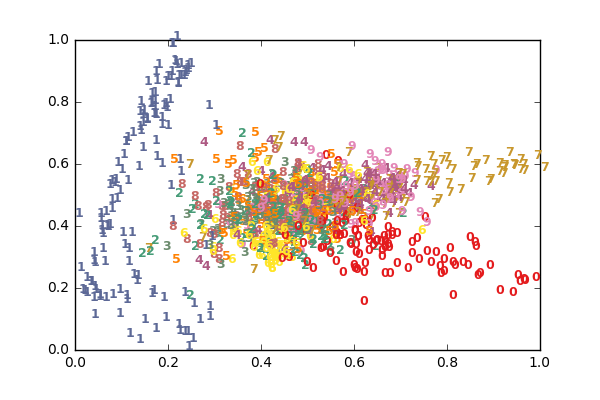
\includegraphics[width=\textwidth]{src/fig10_chebyshev.png}
		\caption{LLE with K = 10}
		\label{fig:src/1figCheby10.png}
	\end{subfigure}
	%(or a blank line to force the subfigure onto a new line)
	\begin{subfigure}[b]{0.28\textwidth}
		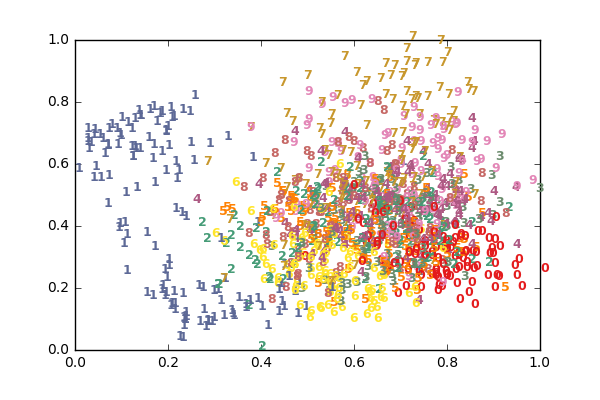
\includegraphics[width=\textwidth]{src/fig50_chebyshev.png}
		\caption{LLE with K = 50}
		\label{fig:src/1figCheby50.png}
	\end{subfigure}
	~ %add desired spacing between images, e. g. ~, \quad, \qquad, \hfill etc. 
	%(or a blank line to force the subfigure onto a new line)
	\caption{Chebyshev metric}\label{fig:fig4}
\end{figure}
\problemAnswer{
\begin{homeworkSection}{(e) Linear manifold interpolation}
%Assume you pick some point in the embedding space. How can you map it back to the original (high dimensional) space? Investigate how well this works for points within and outside the manifold (does it depend on the dimensionality of the embedding space?) Try things like linearly interpolating between two embedding vectors and plot the sequence of images along that line. What happens if you do that in the original space?
See the Reconstruction algorithm in the section implementation for details. We can see in Fig. 5 that the reconstruction is possible for some numbers like 0 and can be hard for numbers like 7. Interpolating between these two numbers in the embedded space also translates to an interpolation in the original space.

\end{homeworkSection}
}
\begin{figure}[h]
	\centering
	\begin{subfigure}[b]{0.16\textwidth}
		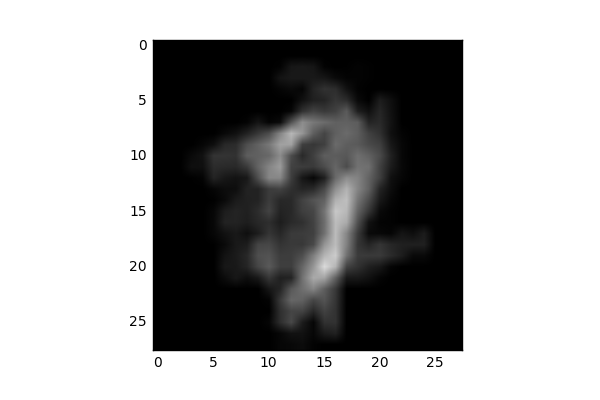
\includegraphics[width=\textwidth]{src/interpolate_0.png}
	\end{subfigure}
	%add desired spacing between images, e. g. ~, \quad, \qquad, \hfill etc. 
	%(or a blank line to force the subfigure onto a new line)
	\begin{subfigure}[b]{0.16\textwidth}
		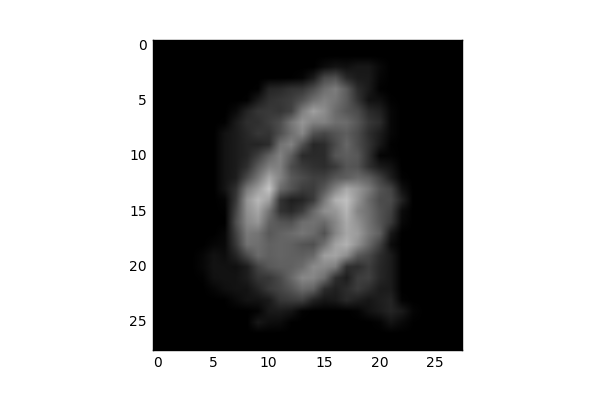
\includegraphics[width=\textwidth]{src/interpolate_1.png}
	\end{subfigure}
	%(or a blank line to force the subfigure onto a new line)
	\begin{subfigure}[b]{0.16\textwidth}
		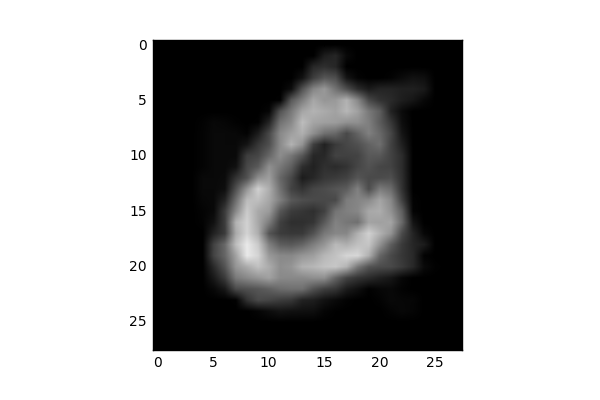
\includegraphics[width=\textwidth]{src/interpolate_2.png}
	\end{subfigure}
   \begin{subfigure}[b]{0.16\textwidth}
   	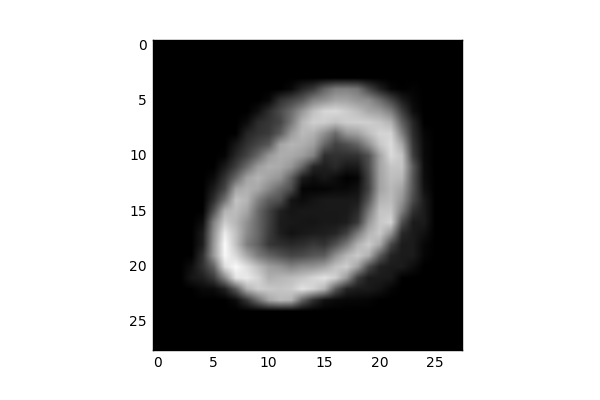
\includegraphics[width=\textwidth]{src/interpolate_3.png}
   \end{subfigure}
	\begin{subfigure}[b]{0.16\textwidth}
		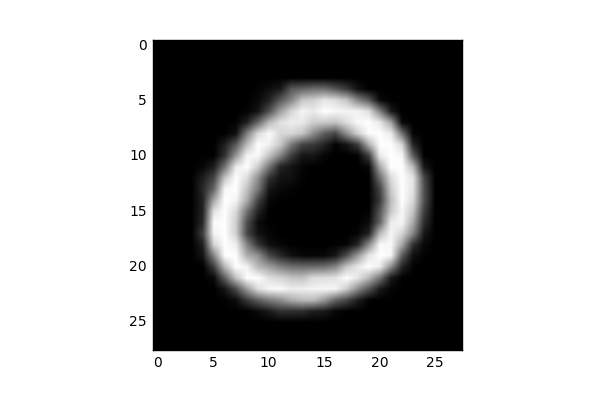
\includegraphics[width=\textwidth]{src/interpolate_4.png}
	\end{subfigure}
	%add desired spacing between images, e. g. ~, \quad, \qquad, \hfill etc. 
	%(or a blank line to force the subfigure onto a new line)
	\caption{Reconstruction of embedded vectors between 7 and 0 (left to right)}
	
	
	\begin{subfigure}[b]{0.16\textwidth}
		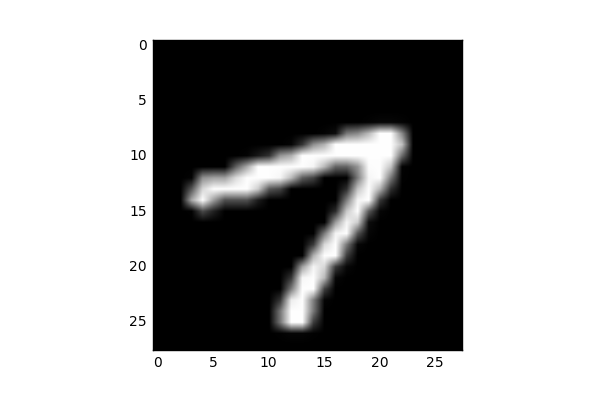
\includegraphics[width=\textwidth]{src/interpolate_original_0.png}
	\end{subfigure}
	%add desired spacing between images, e. g. ~, \quad, \qquad, \hfill etc. 
	%(or a blank line to force the subfigure onto a new line)
	\begin{subfigure}[b]{0.16\textwidth}
		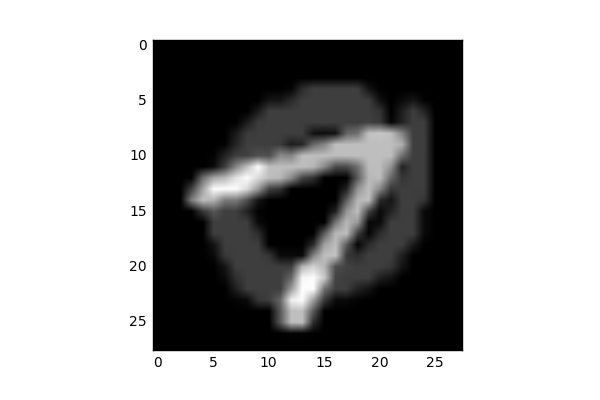
\includegraphics[width=\textwidth]{src/interpolate_original_1.png}
	\end{subfigure}
	%(or a blank line to force the subfigure onto a new line)
	\begin{subfigure}[b]{0.16\textwidth}
		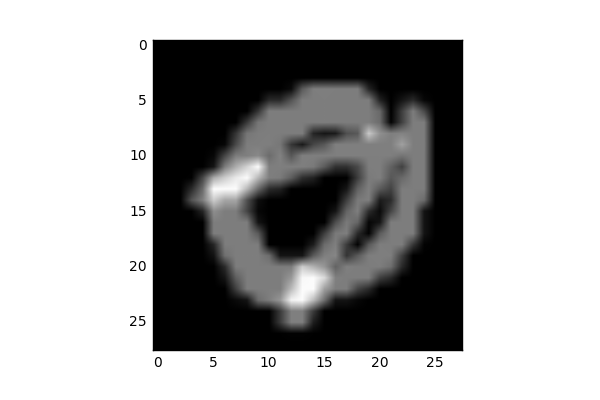
\includegraphics[width=\textwidth]{src/interpolate_original_2.png}
	\end{subfigure}
	\begin{subfigure}[b]{0.16\textwidth}
		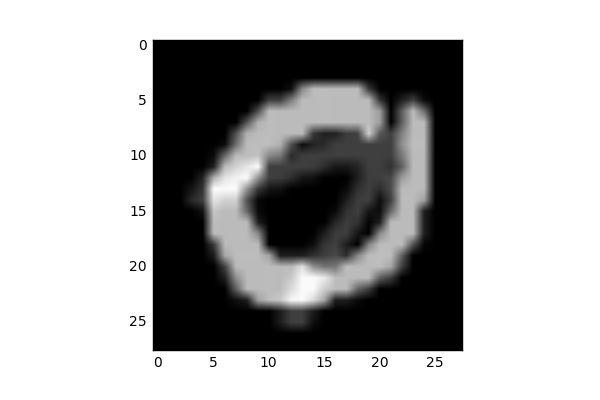
\includegraphics[width=\textwidth]{src/interpolate_original_3.png}
	\end{subfigure}
	\begin{subfigure}[b]{0.16\textwidth}
		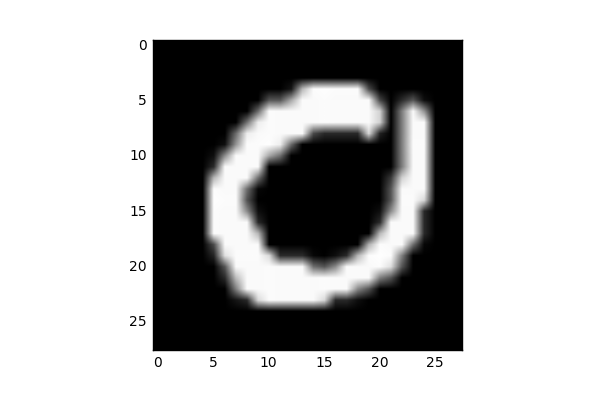
\includegraphics[width=\textwidth]{src/interpolate_original_4.png}
	\end{subfigure}
	\caption{Interpolation in original space from 7 to 0}
\end{figure}





%}
\end{homeworkProblem}
\clearpage

%----------------------------------------------------------------------------------------
\begin{homeworkProblem}[The Implementation]
%In the implementation section you give a concise insight to the practical aspects of this coding exercise. It mainly mentions the optimization methods used to solve the model equations. Did you encounter numerical or efficiency problems? If yes, how did you solve them?
%Provide the link to your git branch of this coding exercise.\newline
%Hard limit: One page

\problemAnswer{ % Answer

\hmwkGitBranch \\

The implementation can be seen in src/code.ipynb. I mostly used the LocallyLinearEmbedding implementation from scikit learn or adapted it. Further I will describe issues I encountered as I worked through the project:

\begin{enumerate}
	\item chosen Parameters \\
	b) I chose n\_neighbors = 30
	\item Efficiency problems (task b) \\
	Because the LLE algorithm has a complexity of $\mathcal{O}(N^2)$ I could not use the full dataset and restricted it to 1200 data points.
\end{enumerate}


$\huge\emph{Reconstruction algorithm}$ \\\\
Given original data matrix $\mathcal{X} \in \mathbf{R}^{nxD}$, embedded space $\mathcal{Y} \in \mathbf{R}^{nxd}$ and a new data point $y_{new} \in \mathbf{R}^{1xd}$ in the embedded space. We reconstruct the point in the original space by the following procedure:
\begin{enumerate}
	\item Find the K nearest neighbors of $y_{new}$. Let's denote them as $NB \in \mathbf{R}^{Kxd}$
	\item Solve the following using a Least Squares approach: $uNB = y_{new}$
	\item For all neighbors in $NB$ find the corresponding points $NB_{orig} \in \mathbf{R}^{KxD}$ in the original space 
	\item Reconstruction: $x_{new} = uNB_{orig}$
\end{enumerate}

}

%LLE has 3 main steps to achieve this goal. Further I'll describe the algorithm with pseudo code:
%\begin{enumerate}
%	\item For each data point $x_i$ find the closest neighbors
%\end{enumerate}

%comments to implementation: 
%b) I chose n\_neighbors to be 30 and used the standard method for measuring distances

%\vspace{10pt}
%\problemAnswer{ % Answer
%Your Answer
%}
\end{homeworkProblem}
\clearpage

%----------------------------------------------------------------------------------------
\begin{homeworkProblem}[Your Page]
%Your page gives you space to include ideas, observations and results which do not fall into the categories provided by us. You can also use it as an appendix to include things which did not have space in the other sections.\newline
%No page limit.

I want cookie. - cookie monster

\vspace{10pt}
\problemAnswer{ % Answer
Your Answer

\hmwkGitBranch % defined in line 5
}
\end{homeworkProblem}
\clearpage

\end{document}

